
\subsection{RESTCompanion}
For a generic and extendable communication protocol we use a separate framework, the RESTCompanion. This framework is not directly related to Social Weaver but is developed parallel and by the author. RESTCompanion provides a web service that can receive tuple messages that contain a specific type code and the message -  we call these parcels. The parcel type includes information about the how the content needs to be processed. For instance we can read from a type code if the parcel is encrypted and what algorithm is used. 

\begin{figure}[h!]
	\begin{verbatim}
		Parcel{type#Integer; message#String}
	\end{verbatim}
\end{figure}

The main feature of RESTCompanion is the different handling for read- and write-parcels and a easy to scale system. It is possible to have multiple RESTCompanion web services instances that listen for incoming messages. Synchronizing happens on server side and clients can just send their messages. This works because there is no direct communication between the client and the web service. After a client sends a message, the message is processed by RESTCompanion. Depending on the operation that follows the client-request, a responder instance will respond to the client. Like for the listening web services there might be severals responders in order to achieve a better scalability. 

RESTCompanion on its own just knows how to retrieve the plain message from a parcel. It does nothing about its content and thats the point where Social Weaver needs to take place. Any system that uses RESTCompanion, needs to implement two methods for processing write and read messages. RESTCompanion redirects a message according to its type to one of the two interfaces. RESTCompanion does not wait or excepts any action after forwarding the message. It depends on the injected system whether the client gets some response. Above we mentioned that synchronization takes place on the server side. To be more accurate synchronizing needs to be implemented inside the system. RESTCompanion does not care about the content and therefore not for the included timestamps as well. 

In case the client send a parcel including some request for information, the system prepares this information and passes it to RESTCompanion including information about encryption and so on. The response is packed up into a parcel and sent back to the client using a not specified responder instance. 

The reader should remember that these parcels are just used in the RESTCompanion context and have nothing to do with the triplets used by Social Weaver. To get a better understanding on this issue lets consider a short example:

\begin{enumerate}
\item Client A creates a Social Weaver triplet for a read request
\item A packs up the triplet into the message part of the triplet and generates a type code that insists that this parcel needs not to be encrypted and includes a reading operation
\item A sends the parcel to a RESTCompanion web service (WS)
\item WS unpacks the parcel and forwards the message (that does not need to be encrypted) to the Social Waver method (S) that implements processing for read-messages (including information about the sender address)
\item S processes the triplet and generates a response
\item S passes that response to RESTCompanion including information about how the message should be encrypted  and the receiver address
\item RESTCompanion creates a parcel from the received information and chooses a responder that sends the parcel to the receiver
\end{enumerate}


\begin{figure}[h!] \centering
		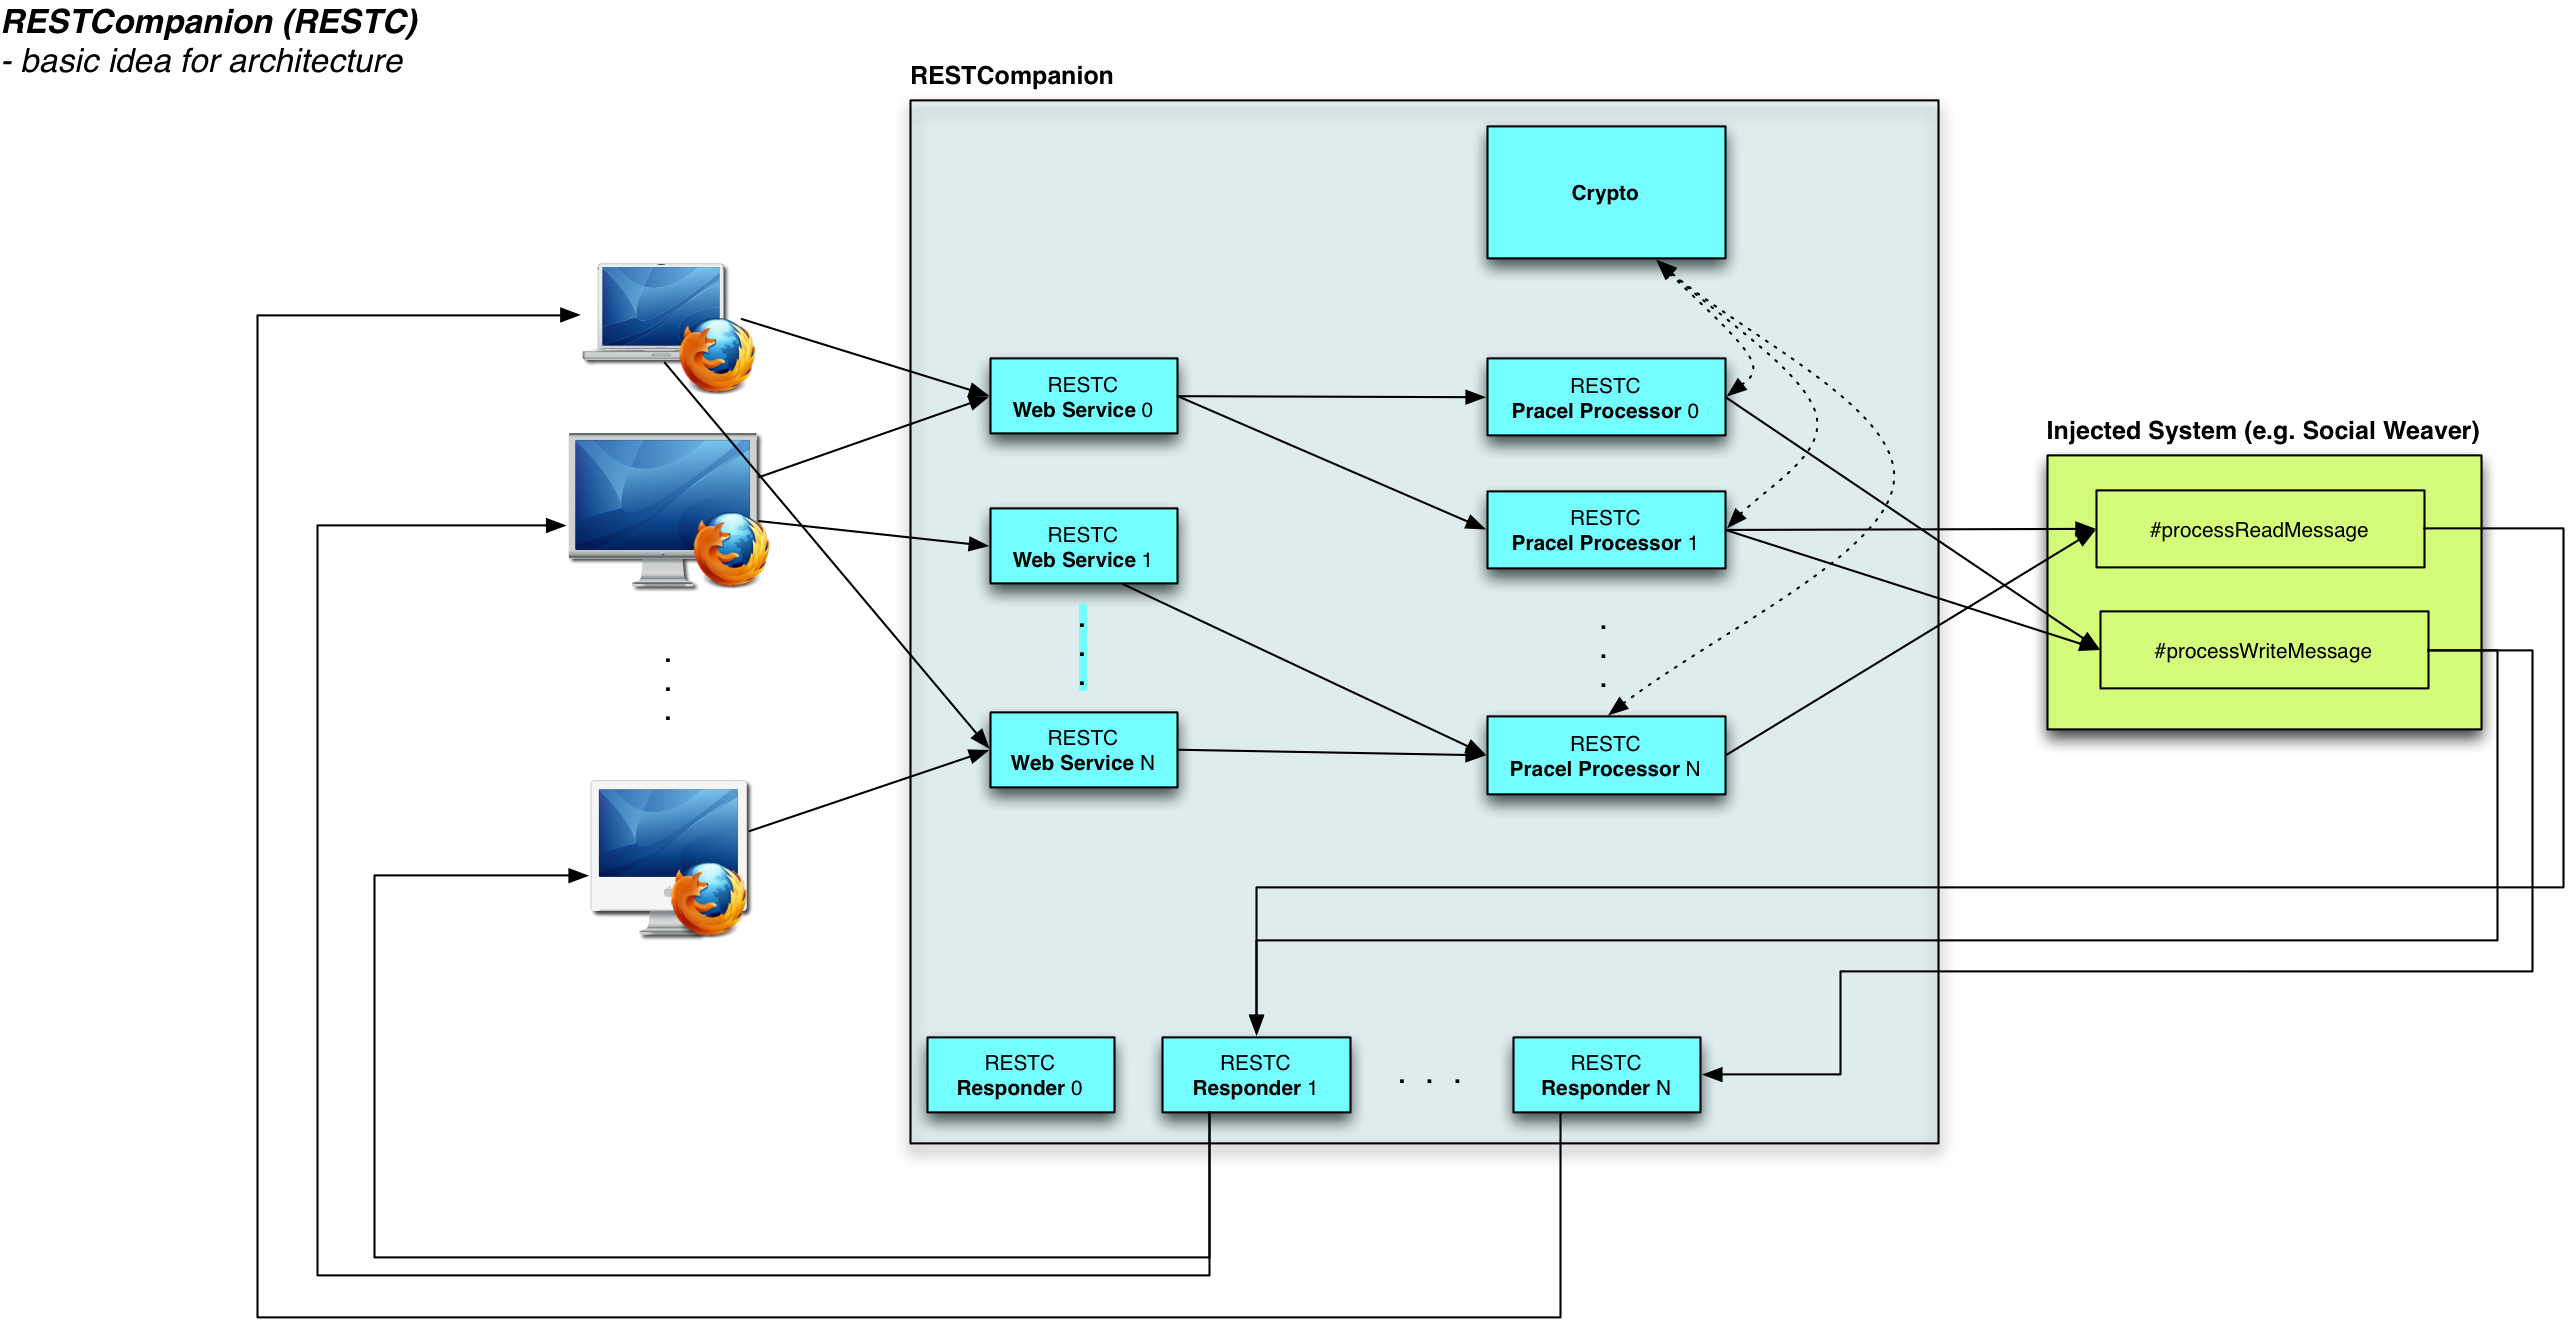
\includegraphics[width=13cm]{images/restcompanion-basic-architecture.png}
		\caption{Basic architecture for RESTCompanion}
\end{figure} 

When we summarize this section it should be clear that RESTCompanion is just used for an extensible  transmission between server and client. Of course clients needs to support the parcel format that is used by the RESTCompanion.

\subsection*{Data format}
What we are discussing in this section is the content-part from the triplets discussed above. The goal is to have an extendable format that uniformly packs any kind of data on its way from plugin to server or from server to plugin. The advantage for using a uniform format is obviously the possibility to add more browser plugins without the need to modify the other modules. 

Our content-parts should contain information about the social media type (whether it is a wiki page, comment box or chat) and its content. We are going to use JSON as data interchange format because is lightweight, easy to read and as an open standard widely distributed.

This could be a example for a content-part that is being sent from a plugin to the server application to notify an update in the comment box:

\begin{lstlisting}[language=json]
{
    "msg_type": "insert",
	"related_element_id": "appointment20121012#eu84ue2",
	"wiki": ""
	"comment": "this is a new comment about the appointment at 2012-10-12"
	"chat" :""
}
\end{lstlisting}

The server application uses the update message to synchronize and persist the new comment. Afterwards it sends a message that might look like this:
\begin{lstlisting}[language=json]
{
    "msg_type": "update",
	"related_element_id": "appointment20121012#eu84ue2",
	"wiki": ""
	"comment": [
		{
			"comment_string": "this is a new comment about the appointment at 2012-10-12",
			"comment_ts": "2012-10-09;-01;14:43:21
			"comment_author": "user11"
		},{
			"comment_string": "this is an older comment about the appointment at 2012-10-12",
			"comment_ts": "2012-10-09;-01;12:32:10
			"comment_author": "user31"
		
		},{
			"comment_string": "this is an old comment about the appointment at 2012-10-12",
			"comment_ts": "2012-10-09;-01;11:02:09
			"comment_author": "user05"
		}
	]
	"chat" :""	
}
\end{lstlisting}

Containing the most recent list of comments this is send to all plugin-clients. The plugin then updates it content in the browser with the latest message from the server.
